\documentclass{report}
\usepackage{url}
\usepackage{todonotes}
\usepackage{booktabs}
\usepackage[utf8]{inputenc}	
\usepackage{float}

\begin{document}

\listoftodos

\tableofcontents

\chapter{Background}

\section{Evasão}
\cite{esclarecimentos_calculos}
\cite{mudanca_calculos}

\subsection{Definição}
Por evasão de discente entenda-se a interrupção de um processo de aprendizado de um discente antes de sua conclusão. Por exemplo, um discente que abandonou o curso de Medicina, na UFC, no qual estava matriculado, pois precisou trabalhar para sustentar sua família e os horários das disciplinas eram incompatíveis com os horários do trabalho. Especificando-se o escopo do processo de aprendizado temos definições mais objetivas de evasão de discente. Por exemplo:
\begin{itemize}
\item Evasão de curso: refere-se ao abandono, pelo discente, de um curso, antes de sua conclusão.
\item Evasão de área de conhecimento: refere-se ao abandono, pelo discente, de um curso, antes de sua conclusão, sem posterior ingresso em curso da mesma área de conhecimento.
\item Evasão de IES: refere-se ao abandono, pelo discente, de um curso, antes de sua conclusão, sem posterior ingresso em curso da mesma IES. 
\item Evasão do ensino: refere-se ao abandono, pelo discente, de um curso, antes de sua conclusão, sem posterior ingresso em outro curso.
\end{itemize}

Esses exemplos não esgotam as possibilidades de definições de evasão de discente, visto ser bastante flexível a definição do escopo do processo de aprendizado. A escolha do escopo a ser considerado deve ser direcionada pelo uso que será feito dos dados calculados a partir da definição de evasão de discente. Por exemplo, para fins de planejamento de políticas de fomento de uma área de conhecimento, pode-se utilizar a definição Evasão de área de conhecimento a fim de verificar se está havendo migração de discentes da área de conhecimento em foco para outras; para fins de comparação, os valores devem ser gerados seguindo a mesma definição, como no caso entre comparações de índices de Evasão de IES entre as IES.

Além do escopo, outro atributo da evasão que pode ser levado em consideração é o agente cuja decisão resultou na interrupção do processo de aprendizado, podendo ser tanto o discente quanto a instituição de ensino.

\todo[inline]{discutir o atributo 'motivo' da evasão}
\todo[inline]{discutir o atributo 'pós evasão'}

De acordo com a literatura analisada \cite{tinto_leaving} \cite{evasao_panorama} a maior parte da evasão de IES ocorre no primeiro ano do discente na instituição.

A evasão de discente configura-se em problema ao considerarmos que o custo x benefício do processo de aprendizado, quando abandonado antes da conclusão, é menor que o esperado. Expectativas podem ser frustradas, como a esperança de formação de corpo técnico para atender às demandas da indústria; recursos podem ficar ociosos, como é o caso de contratação de servidores, a aquisição de equipamentos e a construção de espaços físicos; pode haver diminuição de recursos financeiros da instituição, caso seu orçamento seja vinculado à quantidade de discentes que concluem o processo de aprendizado. 

Atributos do fenômeno evasão de discente:

\begin{enumerate}
\item o agente que interrompeu o processo
\item o discente
\item o curso
\item a instituição de ensino
\item o tempo cursado
\item o motivo
\end{enumerate}

\subsection{Indicadores de evasão}

\subsubsection{Taxa de sucesso}

Definido com esse nome em \cite{indicadores_TCU} e com o nome "Taxa de titulação" em \cite{mudanca_calculos}, esse indicador é a razão entre a quantidade de discentes concluintes efetivos e a quantidade de concluintes esperados, considerando prazo esperado de conclusão.
Este indicador abstrai a ocorrência de ocupação, via transferência, de vaga ociosa por evasão; considera apenas as conclusões no prazo esperado, podendo gerar dados inesperados, como percentuais acima de 100\%, indicando haver se formado no ano em questão mais discentes que o esperado, consequência, por exemplo, de discentes atrasados ou de discentes adiantados.
\begin{equation}
\frac{Nº\ de\ diplomados(N_{DI})}{Nº\ total\ de\ alunos\ ingressantes}
\end{equation}

\todo[inline]{discutir as vantagens e desvantagens dessa métrica e como interpretá-la}

\subsubsection{Evasão anual}

Definido em \cite{esclarecimentos_calculos} e \cite{mudanca_calculos}, é a razão entre a quantidade de rematrículas realizadas e a quantidade de rematrículas esperadas.
\begin{equation}
1 - \frac{M(n) - Ig(n)}{M(n-1) - Eg(n-1)}
\end{equation}
\begin{itemize}
\item $M(n)$: quantidade de matrículas na unidade de tempo $n$
\item $Eg(n)$: quantidade de egressos na undiade de tempo $n$
\item $Ig(n)$: quantidade de ingressantes na unidade de tempo $n$
\end{itemize}

Para derivar essa taxa, basta notarmos as seguintes equações e respectivos significados:
\begin{enumerate}
\item 
\begin{equation}
M(n) = E(n) + X(n) + Eg(n)
\end{equation}
significando que a quantidade de matrículas em determinada unidade de tempo $n$ é composta pelas quantidades de matrículas de discentes que evadirão em $n$, de discentes que persistirão, isto é, se matricularão em $n+1$, e de discentes que se diplomarão ao fim de $n$.
\item 
\begin{equation}
M(n) = X(n-1) + Ig(n)
\end{equation}
significando que a quantidade de matrículas em determinada unidade de tempo $n$ é composta pelas quantidades de matrículas de discentes que se matricularam em $n$ e em $n-1$, ou seja, que persistiram de $n-1$ a $n$, e de discentes que ingressaram em $n$.
\end{enumerate}

Fazendo as devidas manipulações nas equações, chegamos na equação de quantidade de evasões ao fim de determinada unidade de tempo:
\begin{equation}
E(n) = [M(n) - Eg(n)] - [M(n+1) - Ig(n+1)]
\end{equation}
Podendo ser interpretada como a diferença de quantidade máxima de discentes persistindo e a quantidade efetiva de discentes que persistiram.

A fórmula da evasão anual pode ser então definida como a proporção entre a quantidade de evasões em uma unidade de tempo e a quantidade máxima de discentes persistindo naquela unidade de tempo.

A definição de evasão anual até então analisada refere-se à evasão de cursos, de forma que um discente que tenha mudado de curso na mesma IES terá ao mesmo tempo contabilizados sua matrícula no período anterior($M(n-1)$) e como ingressante($Ig(n)$).

\todo{analisar o ciclo de vida de discente e derivar os indicadores}
Para a evasão anual de IES, é proposta a seguinte definição:
\begin{equation}
1 - \frac{M(n) - [Ig(n) - ITC(n)]}{M(n-1) - Eg(n-1)}
\end{equation}
\begin{itemize}
\item $ITC(n)$: quantidade de ingressantes no ano $n$ com forma de ingresso transferência interna
\end{itemize}

Já para a evasão anual do sistema, a ser aplicada a dados de várias, se possível todas, IES, a definição proposta é:
\begin{equation}
1 - \frac{M(n) - [Ig(n) - ITC(n) - ITIES(n)]}{M(n-1) - Eg(n-1)}
\end{equation}
\begin{itemize}
\item $ITIES(n)$: quantidade de ingressantes no ano $n$ com forma de ingresso transferência externa
\end{itemize}

\todo[inline]{discutir as vantagens e desvantagens dessa métrica e como interpretá-la}
\todo[inline]{calcular indicadores para a UFC}

\subsection{Consequências}

Sob a perspectiva de que o processo de aprendizado é um investimento e que o resultado esperado é a sua conclusão, o fenômeno evasão de discente pode ser considerado um problema: para a sociedade, com a frustração da expectativa de formação de profissionais e pesquisadores qualificados; para a instituição de ensino, caso tenha realizado investimentos em infraestrutura e em recursos humanos para atender a uma quantidade esperada de discentes ativos maior que a real, ocorrendo desperdício de recursos; caso seu orçamento seja ou função da quantidade de discentes ativos, no caso das instituições de ensino particulares, ou função da quantidade de discentes diplomados, no caso das instituições de ensino superior públicas\todo{validar o impacto da evasão no orçamento das IFES}; para o indivíduo que investiu tempo, dinheiro e dedicação, mas não terá os benefícios da conclusão da graduação, crítica no caso das profissões que exigem, para serem exercidas, diploma de graduação.

\subsection{Causas}

\subsubsection{Fonte: Instituto Lobo}
De acordo com o Instituto Lobo\cite{evasao_panorama2}, as causas mais comuns de evasão do sistema de ensino superior no Brasil são:

\begin{enumerate}

\item \textbf{Baixa qualidade da educação básica brasileira}: mensurada pelos exames internacionais\todo{pesquisar indicadores de qualidade da educação básica brasileira}.

\item \textbf{Baixa eficiência e o diploma do ensino médio}: que não garante a suficiência de competência do candidato ao ensino superior, criando dificuldades de adaptação e acompanhamento do curso.

\item \textbf{Limitação das políticas de financiamento ao estudante}: mesmo com FIES e PROUNI são insuficientes\todo{pesquisar discussão sobre limitações nas políticas de financiamento}, e para alunos do setor público que, em certos casos, deixam de estudar por não terem meios financeiros para se manterem.

\item \textbf{Escolha precoce da especialidade profissional}: incorre aqui a existência de grande quantidade de cursos de graduação(mais de 200), muito especializados. A título de exemplo, o curso de Direito no Brasil tem duração de 5 anos e ao fim já garante o exercício profissional ao formado após o exame da Ordem, quando em outros países esse curso é uma espécie de pós-graduação.

\item \textbf{Dificuldade de mobilidade estudantil}: composta pela dificuldade de transferência entre IES e pela dificuldade de aproveitamento de créditos. A tendência em países desenvolvidos é a unificação de currículos, que diminui tais dificuldades.

\item \textbf{Rigidez do arcabouço legal e das exigências para autorização/reconhecimento de cursos}: há um risco de inovações nos projetos pedagógicos não serem aprovadas pela Comissão de autorização e/ou reconhecimento.

\item \textbf{Falta de pressão para combater a evasão}: em virtude da cultura acadêmica, pela qual um curso nasce e responde às necessidades e visão dos docentes, em especial das IES públicas(e até de sindicados, associações de classe e profissionais que trabalham muitas vezes pela reserva de mercado e manutenção do status quo).

\item \textbf{Legislação sobre inadimplência no Brasil}: uma excrecência demagógica que educa para o calote, favorece o acúmulo de dívidas pelo aluno e a Evasão das IES privadas.

\item \textbf{Enorme quantidade de docentes despreparados para o ensino e para lidar com o aluno real}: o que ocorre, entre muitas razões, pela falta de formação didático-pedagógica de vários deles e pela acomodação oriunda da estabilidade precoce de muitos(por força legal nas IES públicas e de fato nas IES privadas), tudo isso somado à dificuldade de cobrança de desempenho e à pequena valorização do ensino nos planos e promoções de carreira docente, com valorização quase exclusiva da produção científica

\item \textbf{Inadaptação ao estilo do ensino superior}

\item \textbf{Dificuldade financeira}

\item \textbf{Irritação com a precariedade dos serviços oferecidos pela IES}

\item \textbf{Decepção com a pouca motivação e atenção dos professores}

\item \textbf{Dificuldades com transporte, alimentação e ambientação na IES}

\item \textbf{Mudança de curso}

\item \textbf{Mudança de residência}

\end{enumerate}

Em \cite{evasao_panorama2} são apresentados modelos teóricos que tentam explicar a evasão e são precursores do trabalho de Vincent Tinto, indicado com um dos maiores especialistas em evasão.

\begin{itemize}
\item \textbf{Modelos psicológicos}: Belief, attitude, intention and behavior: An introduction to theory and research(Ajzen 1975); A psychological model of student persistence(Ethington 1990).

\item \textbf{Modelos de integração estudante - instituição}: baseia-se no fato de que a integração do aluno com a IES é fundamental para a sua permanência.\todo{é citado Spady 1975, mas não achei a referência...}
\end{itemize}

É citada frase de T.E.Corts, ex-presidente da Samford University, que copio em parte:
\begin{quote}
Algumas pesquisas indicam que estudantes não abandonam faculdades por grandes razões, mas pelo acúmulo de pequenas razões que destroem suas justificativas de escolha de uma instituição.
\end{quote}

\subsubsection{Fonte: Opinião de docentes e de coordenadores acerca do fenômeno da evasão discente dos cursos de graduação da Universidade Federal do Ceará(UFC)}

No trabalho \cite{andriola} são apresentados os \textbf{resultados de pesquisa feita com uma amostra(tamanho 86 de um universo de tamanho 412) de discentes evadidos no período de 1999 e 2000 acerca dos motivos que os levaram a abandonar os cursos}. Os seguintes fatores foram apresentados:

\begin{enumerate}

\item Incompatibilidade entre horários de trabalho e de estudo(destacado por 39.4\% dos evadidos).

\item Aspectos familiares(por exemplo: necessidade de dedicar-se aos filhos menores) e desmotivação com os estudos(justificado por 20\% dos evadidos).

\item Precariedade das condições físicas do curso ou inadequação curricular(mencionado por 10\% dos evadidos).

\end{enumerate}


\subsubsection{Vincent Tinto}

Em \cite{evasao_panorama2} é citada a crítica de Tinto à formação didático-pedagógica dos professores do ensino superior; sua ênfase na interação do aluno na IES; seu alerta para que sejam analisadas as causas em todos os envolvidos no processo, e não apenas no aluno; a maior concentração de evasão no primeiro ano; a preocupação com a diminuição na qualidade da educação dos ingressantes, recomendando a adoção de programas específicos para os perfis dos novos aunos; e o engano que pode ser causado por aceitarmos a justificativa de problema financeiro para a evasão, quando outras causa podem ter tido maior influência.

Em \cite{tinto_leaving} Vincent Tinto explora o problema da evasão de discentes primeiro analisando o perfil dos discentes ingressantes e evadidos, depois analisando estudos sobre o fenômeno e desenvolvendo sua própria teoria, finalizando com uma discussão sobre as ações que as instituições podem executar para reduzir o problema.

\textbf{p. 1}

Dos 2.4 milhões de ingressantes em 1993, 1.5 milhões abandonarão a primeira instituição de ingresso, sem se diplomarem; desses, 1.1 milhões não retornarão ao ensino superior.

Relação entre diploma e reward - apresenta o salário anual médio, em 1989, de um profissional com e sem diploma, apontando ser relevante a diferença, mas alertando para que isso não quer dizer que não há benefícios caso o processo seja interrompido antes da conclusão(conhecimento foi adquirido, por exemplo).

\textbf{p. 2}

Apresenta uma informação que também aparece nos documentos do Instituto Lobo: que a oferta e ocupação de vagas, em determinado momento, saturou, fazendo com que o foco das ações das instituições para geração de renda passasse do marketing para aumento de ingressos para aquelas que buscassem aumentar a retenção dos discentes já ingressos.

\textbf{p. 3}

Alerta para que o problema é complexo.

Alerta para que a evasão, do ponto de vista dos discentes, nem sempre é vista como algo negativo. Lembrar que o processo não concluído não implica em ausência de benefícios; além do caso de escolha errada de curso(vocação).

Alerta para a dificuldade em isolar os fatores que contribuem para a evasão e a retenção, de forma que é complicado replicar resultados entre instituições.

\textbf{p. 4}

Alerta, novamente, que os fatores envolvidos na evasão/retenção estão distribuídos no contexto e não concentrados em poucas entidades.

\textbf{p. 5}

Alerta para que, antes de serem executadas ações relacionadas a evasão, é importante que a instituição analise quais os objetivos busca alcançar com tais ações, principalmente em vista das diversas definições de evasão(quer diminuir a evasão da instituição? de curso? transferência por falta de vocação? etc).

A estrutura do livro segue:

\begin{enumerate}

\item ch02: analisa o perfil dos ingressantes e evadidos

\item ch03: analisa estudos até então desenvolvidos
 
\item ch04: desenvolve uma teoria para o fenômeno

\item ch05: discute ações que podem ser executadas para reduzir o problema

\end{enumerate}

\todo[inline]{continuar resumo do Leaving College}

\subsection{Soluções}

\subsubsection{Fonte: Instituto Lobo}

Em \cite{evasao_panorama2} são apresentados "Sete pontos para baixar a evasão":

\begin{enumerate}

\item Estabelecer um grupo de trabalho encarregado de reduzir a evasão.

\item Avaliar as estatísticas da evasão.

\item Determinar as causas da evasão.

\item Estimular a visão da IES centrada no aluno.

\item Criar condições que atendam aos objetivos que atraíram os alunos.

\item Tornar o ambiente e o trânsito na IES agradáveis aos alunos.

\item Criar programa de aconselhamento e orientação dos alunos.

\end{enumerate}

E na seção "Conclusões e recomendações sobre a evasão no ensino superior brasileiro":

\begin{enumerate}

\item O problema da evasão deve ser discutido com todos os envolvidos no processo.

\item O problema da evasão deve ser combatido em todos os niveis, não apenas no operacional.

\item São necessários dados confiáveis e organizados para se realizar bons planejamentos.

\item É necessário buscar a integração das áreas acadêmicas e administrativo-financeira das IES para que ambas caminhem juntas no combate à evasão.

\item A adoção de equipe técnica para estudar e acompanhar o fenômeno deve ser acompanhada do apoio e do trabalho de todos da instituição.

\item "O comprometimento com o sucesso do aluno implica na coragem de buscar medidas, nem sempre simpáticas aos professores e alunos, para que se garanta o aprendizado e a medição desse aprendizado, tais como provas elaboradas por outros professores, avaliações de desempenho com consequências etc."

\item "Afirmar que as questões financeiras(da IES e do aluno) não dizem respeito à academia, é ignorar que tudo o que afeta a missão de uma IES envolve, necessariamente, a academia."

\item "No fundo, todos os problemas de uma IES passam, necessariamente, pela GESTÃO. A gestão universitária é uma profissão para a qual é preciso treinar os professores e profissionais que a ela se dedicam, ou pensam/se propõem a se dedicar e, por isso, os gestores das IES precisam ser capacitados para entender e combater a evasão"

\item "Não se pode ensinar ao aluno a ser um profissional e um cidadão comprometido quando uma IES demonstra amadorismo em seus processos e descuidos em relação ao seu maior compromisso: o auno, que é a razão de ser de uma IES!"

\end{enumerate}

\subsubsection{Fonte: Vincent Tinto}
\todo[inline]{soluções apontadas por Vincent Tinto}

\subsubsection{Fonte: Opinião de docentes e de coordenadores acerca do fenômeno da evasão discente dos cursos de graduação da Universidade Federal do Ceará(UFC)}

No trabalho \cite{andriola} são apresentados os resultados de pesquisa, iniciada em 2004, feita com 21 coordenadores e 52 docentes da UFC, com questionário abordando os seguintes temas:
\begin{itemize}
\item Resgate da função do professor orientador.
\item Informações necessárias aos futuros universitários acerca do curso escolhido.
\item Opinião dos coordenadores acerca do envolvimento docente no ensino de graduação.
\item Contribuição da atual administração da UFC para a melhoria do desempenho das coordenações.
\item Papel da gestão central, dos coordenadores e dos docentes no combate ao fenômeno da evasão.
\end{itemize}
(o autor alerta para que a amostragem foi orientada pela disponibilidade dos docentes e dos coordenadores, e pela facilidade de obtenção dos dados).

\textbf{Sobre a função do professor orientador.}

87\% dos coordenadores e 74\% dos docentes foram favoráveis à função do professor orientador. 20\% dos coordenadores apontaram os seguintes requisitos como primordiais para a implantação dessa atividade:

\begin{itemize}
\item Preparação do corpo docente.
\item Disponibilidade de tempo para tal atividade, formalmente estabelecida enquanto atividade docente.
\item Compromisso formalmente assumido por todos os docentes visando o acompanhamento direto e sistemático aos discentes.
\end{itemize}

16.2\% dos docentes destacaram que para a realização de um trabalho de orientação contínua é necessário:

\begin{itemize}
\item Preparação do corpo docente.
\item Disponibilização de tempo e de recursos materiais.
\item Atribuição de pontos na Gratificação de Estímulo à Docência(GED).
\end{itemize}

12.2\% dos docentes foram desfavoráveis à função de professor orientador, apresentando os seguintes motivos:

\begin{itemize}
\item Número insuficiente de docentes.
\item Falta de tempo, por já estarem envolvidos em muitas atividades.
\item Recursos insuficientes para a realização desse tipo de trabalho.
\end{itemize}

\textbf{Sobre informações necessárias aos discentes.}

Para 92\% dos coordenadores e 81.1\% dos docentes entrevistados, é papel da coordenação fornecer informações sobre o curso, através de ações como:

\begin{itemize}
\item Realização de seminários, disciplinas introdutórias, palestras e outros eventos.
\item Visita às escolas de ensino médio.
\item Divulgação de informações pela internet e por meio de trabalho coletivo entre as coordenações e as Pró-Reitorias de Graduação e de Assuntos Estudantis.
\item Distribuição de folhetos no período das inscrições para o vestibular.
\end{itemize}

\textbf{Sobre o envolvimento docente no ensino de graduação.}

Para 41.1\% dos coordenadores e 23.5\% dos docentes entrevistados, o envolvimento dos docentes no ensino de graduação é insatisfatório. Foi destacado pelos entrevistados que muitos docentes priorizam o ensino de pós-graduação e a pesquisa.

\textbf{Sobre a contribuição da atual administração da UFC para melhorar o desempenho das coordenações.}

As seguintes ações foram apresentadas:

\begin{itemize}
\item Urgência na efetivação de ações visando melhoria na infra-estrutura.
\item Compreensão das causas da evasão discente visando a combatê-la.\todo{motivação para mineração de dados}
\item Importância do apoio da Reitoria e da Pró-Reitoria de Graduação.
\item Informação aos vestibulandos acerca de aspectos básicos dos cursos de graduação.
\item Necessidade de maior autonomia e poder de decisão.
\end{itemize}

\textbf{Sobre o papel da gestão central, dos coordenadores e dos docentes no combate ao fenômeno da evasão.}

As seguintes ações foram apresentadas:

\begin{itemize}
\item Maior apoio às atividades de estágio, monitoria, pesquisa e extensão
\item Melhorar a estrutura física dos cursos, no que diz respeito às saldas de aula, laboratórios e recursos áudio-visuais
\item Aumentar a oferta de cursos noturnos e a qualidade do ensino e do projeto político-pedagógico.
\item Promoção de seminários destinados aos egressos do ensino médio, com vistas a informá-los acerca dos cursos, das carreiras profissionais, dos eventos acadêmico-científicos, dos estágios, da pós-graduação e de bolsas.
\item Acompanhar e orientar os discentes de modo sistemático e institucionalizado.\todo{motivação para mineração de dados}
\item Flexibilizar a grade curricular, rever critérios de pré-requisitos, viabilizar decisões colegiadas nas coordenações, cobrar dos docentes maior comprometimento com o ensino.
\item Melhorar a formação dos docentes para o papel de educador.
\item Tornar as aulas mais interessantes e unir teoria e prática.
\item Melhorar a avaliação de desempenho dos alunos; incrementar o combate às dificuldades de aprendizagem; apoiar as iniciativas das coordenações por mais investimentos para as bibliotecas e para a aquisição de equipamentos didáticos.
\end{itemize}

\textbf{Sobre como as coordenações poderiam executar atividades de apoio e incentivo aos discentes.}

45\% dos coordenadores ressaltaram a conversa com os pretensos a abandonar o curso para, assim, tentar reverter a situação.\todo{motivação para predição de evadido} 25\% dos coordenadores enfatizaram que é importante a contribuição das coordenações na melhoria da qualidade do ensino e do projeto político-pedagógico dos cursos, ressaltando que para tanto as coordenações necessitam de maior aporte orçamentário, além de estreitar parcerias com as Pró-Reitorias de Graduação e de Assuntos Estudantis.

\textbf{Sobre a atuação docente.}

31.8\% dos coordenadores indicaram que é preciso haver maior compromisso dos docentes com o ensino de graduação, visto que muitos estão mais envolvidos com o ensino da pós-graduação e com pesquisas. 18.1\% dos coordenadores destacaram que os docentes poderiam orientar e ampliar o incentivo dos discentes para a realização de atividades relevantes para a vida acadêmica. 9\% dos coordenadores entrevistados apresentaram as seguintes atividades: adequada avaliação do desempenho dos alunos, combate às dificuldades de aprendizagem, melhoria da didática e melhoria da relação professor-aluno.

\textbf{Sobre a necessidade de trabalhar e incompatibilidade de horários, como motivo para evasão.}

Os entrevistados apresentaram as seguintes soluções:

\begin{itemize}
\item Aumento da oferta de bolsas e de estágios.
\item Concentração das disciplinas em apenas um turno.
\item Aumento da oferta de cursos noturnos.
\end{itemize}


\section{Fonte: site da UFC}

\url{http://ufc.br/a-universidade}

"A Universidade Federal do Ceará é uma autarquia vinculada ao Ministério da Educação. Nasceu como resultado de um amplo movimento de opinião pública. Foi criada pela Lei nº 2.373, em 16 de dezembro de 1954, e instalada em 25 de junho do ano seguinte.

No início, sob a direção de seu fundador, Prof. Antônio Martins Filho, era constituída pela Escola de Agronomia, Faculdade de Direito, Faculdade de Medicina e Faculdade de Farmácia e Odontologia.

Sediada em Fortaleza, Capital do Estado, a UFC é um braço do sistema do Ensino Superior do Ceará e sua atuação tem por base todo o território cearense, de forma a atender às diferentes escalas de exigências da sociedade.

A Universidade é composta de sete campi, denominados Campus do Benfica, Campus do Pici e Campus do Porangabuçu, todos localizados no município de Fortaleza (sede da UFC), além do Campus de Sobral, Campus de Quixadá, Campus de Crateús e Campus de Russas.

A Universidade Federal do Ceará, que há mais de 50 anos mantém o compromisso de servir à região, sem esquecer o caráter universal de sua produção, chega hoje com praticamente todas as áreas do conhecimento representadas em seus campi." 

\section{Fonte: Anuário estatístico 2014 base 2013}

\cite{anuario_2014_base_2013}

\subsection{Objetivos institucionais}

A UFC orienta sua atuação permanentemente no sentido de alcançar os seguintes objetivos:
\begin{enumerate}
\item
Promover a formação humana e profissional de seus estudantes, preparando-os para uma atuação responsável e construtiva na sociedade;
\item
Fomentar a geração de conhecimentos voltados para o desenvolvimento sustentável do Ceará e do Nordeste;
\item
Impulsionar o desenvolvimento, a produção e a preservação da cultura e das artes, com ênfase para as manifestações regionais.
\item
Promover a interação com a sociedade, através da difusão científica, tecnológica, artística e cultural e do desenvolvimento comunitário, sintonizados com as demandas sociais;
\item
Incentivar a capacitação permanente dos quadros docente e técnico-administrativo;
\item
Intensificar e ampliar as relações de parceria e intercâmbio com instituições nacionais e estrangeiras, governamentais e não governamentais;
\item
Buscar a profissionalização da gestão administrativa, apoiada em processos de planejamento e avaliação, executada com base em modelo organizacional flexível, eficiente e eficaz;
\item
Exercitar permanentemente o instituto da autonomia universitária superando restrições e estabelecendo novos parâmetros na gestão e nas relações institucionais;
\item
Assegurar a qualidade no desenvolvimento de todas as ações administrativas e acadêmicas;
\item
Distinguir-se como referência regional pela excelência acadêmica de suas ações nas áreas do ensino, geração do conhecimento e prestação de serviços à população, bem como na produção de arte e cultura.
\end{enumerate}
\textbf{p. 10}

\subsection{Lema}

“O universal pelo regional” é o lema da UFC, instituição que busca centrar seu compromisso na solução dos problemas locais, sem esquecer o caráter universal de sua produção.
\textbf{p. 11}

\subsection{Missão}

A missão da Universidade é formar profissionais da mais alta qualificação, gerar e difundir conhecimentos, preservar e divulgar os valores éticos, científicos, artísticos e culturais, constituindo-se em instituição estratégica para o desenvolvimento do Ceará, do Nordeste e do Brasil.
\textbf{p. 11}

\subsection{Visão}

\underline{Consolidar-se como instituição de referência no ensino de graduação} e pós-graduação (stricto e lato sensu), de preservação, geração e produção de ciência e tecnologia, e de integração com o meio, como forma de contribuir para a superação das desigualdades sociais e econômicas, por meio da promoção do desenvolvimento sustentável do Ceará, do Nordeste e do Brasil.
\textbf{p. 11}

\subsection{Estrutura organizacional e instâncias de decisão}

A Universidade Federal do Ceará, criada em 1954, é uma instituição federal de ensino superior, constituída como autarquia educacional de regime especial e vinculada ao Ministério da Educação.

A UFC é regida administrativa e juridicamente de acordo com seu Estatuto, Regimento Geral e Regimento Interno de suas diversas unidades. A administração e coordenação das atividades universitárias são exercidas em dois níveis: 

\begin{itemize}
\item Administração Superior
\item Administração Acadêmica
\end{itemize}

\subsubsection{Administração Superior}

A Administração Superior da Universidade é exercida através dos seguintes órgãos:

\subsubsection{Conselho Universitário(CONSUNI)}

Função: O Conselho Universitário (órgão colegiado com representação estudantil) é o órgão superior deliberativo e consultivo para traçar a política universitária e decidir em matéria de administração, inclusive gestão econômico-financeira.


\subsubsection{Conselho de Ensino, Pesquisa e Extensão(CEPE)}

Função: O Conselho de Ensino, Pesquisa e Extensão (órgão colegiado com representação estudantil) é o órgão superior deliberativo e consultivo da Universidade, em matéria de ensino, pesquisa e extensão.

\subsubsection{Conselho de Curadores}

Função: O Conselho de Curadores (órgão colegiado com representação estudantil) é o órgão com atribuições de fiscalização econômico-financeira.

\subsubsection{Reitoria}

Órgão Superior executivo que tem por finalidade planejar, organizar, coordenar, dirigir e controlar as atividades de administração em geral, de planejamento, de assuntos estudantis, de graduação, de pós-graduação, de pesquisa e de extensão no âmbito da Universidade.

Estrutura Orgânica da Reitoria 
\begin{enumerate}
\item Órgãos de Assistência Direta ao Reitor
	\begin{itemize}
	\item Gabinete
	\item Procuradoria Geral
	\end{itemize}
\item Órgãos de Assessoramento ao Reitor
	\begin{itemize}
	\item Coordenadoria de Comunicação Social e Marketing Institucional
	\item Coordenadoria de Assuntos Internacionais
	\item Secretaria dos Órgãos Deliberativos Superiores
	\item Ouvidoria Geral
	\item Auditoria Interna
	\item Coordenadoria de Concursos
	\item Editora da UFC
	\end{itemize}
\item Órgãos de Planejamento e Administração
	\begin{itemize}
	\item Pró-Reitoria de Planejamento
	\item Pró-Reitoria de Administração
	\item Pró-Reitoria de Gestão de Pessoas
	\item Superintendência de Infraestrutura
	\item Superintendência dos Hospitais Universitários
	\end{itemize}
\item Órgãos de Atividades Específicas
	\begin{itemize}
	\item Pró-Reitoria de Graduação
	\item Pró-Reitoria de Extensão
	\item Pró-Reitoria de Pesquisa e Pós-Graduação
	\item Pró-Reitoria de Assuntos Estudantis
	\end{itemize}
\item Órgãos Suplementares
	\begin{itemize}
	\item Casa de José de Alencar
	\item Biblioteca Universitária
	\item Imprensa Universitária
	\item Secretaria de Acessibilidade - UFC Inclui
	\item Secretaria de Tecnologia da Informação
	\item Seara da Ciência Museu de Arte da UFC – MAUC
	\item Secretaria de Cultura Artística (SECULT-ARTE-UFC)
	\item Memorial da UFC
	\end{itemize}
\end{enumerate}     

\subsubsection{Administração Acadêmica}

Os departamentos são coordenados por unidades, com a denominação de Centros ou Faculdades.
Os departamentos constituem a menor fração da estrutura universitária, para todos os efeitos de organização administrativa e didático-científico, bem como de distribuição de pessoal, exceto nos casos dos campi de Sobral, Cariri, Quixadá, Russas, Crateús e dos Institutos de Ciências do Mar – LABOMAR, Cultura e Arte – ICA, Universidade Virtual – UFC Virtual e de Educação Física e Esportes - IEFES, nos quais as unidades acadêmicas são constituídas pelas coordenações dos cursos.

\subsubsection{Centros, Faculdades e Institutos}

\begin{enumerate}
\item Centro de Ciências
\item Centro de Humanidades
\item Centro de Tecnologia
\item Centro de Ciências Agrárias
\item Faculdade de Medicina
\item Faculdade de Farmácia, Odontologia e Enfermagem
\item Faculdade de Direito
\item Faculdade de Educação
\item Faculdade de Economia, Administração, Atuariais, Contabilidade e Secretariado Executivo
\item Instituto de Ciências do Mar (LABOMAR)
\item Instituto de Cultura e Arte (ICA)
\item Instituto de Educação Física e Esportes (IEFES)
\item Instituto Universidade Virtual – UFC Virtual
\end{enumerate}

\subsubsection{Unidades do interior do estado}

\begin{enumerate}
\item Campus da UFC em Sobral
\item Campus da UFC no Cariri
\item Campus da UFC em Quixadá
\item Campus de Russas
\item Campus de Crateús
\end{enumerate}

Deve-se observar que a administração superior criou uma estrutura acadêmico-administrativa diferenciada nas unidades acadêmicas do interior do estado. A opção foi de não criar departamentos; portanto, as unidades acadêmicas são os próprios campi, constituídos pelas coordenações dos cursos existentes.
A administração dos campi do interior do Estado, dos institutos e dos centros ou faculdades é exercida pelos seguintes órgãos: 

\begin{itemize}
\item Conselho do Campus (Unidades do Interior do Estado)
\item Conselho de Centro ou Conselho Departamental (nas Faculdades)
\item Diretoria
\item Vice-Diretoria
\item Secretaria
\item Coordenação de Cursos de Graduação
\item Coordenação de Cursos de Pós-Graduação
\end{itemize}

\textbf{p. 11 a 13}

\subsection{Orçamento da UFC}

\begin{figure}[H]
	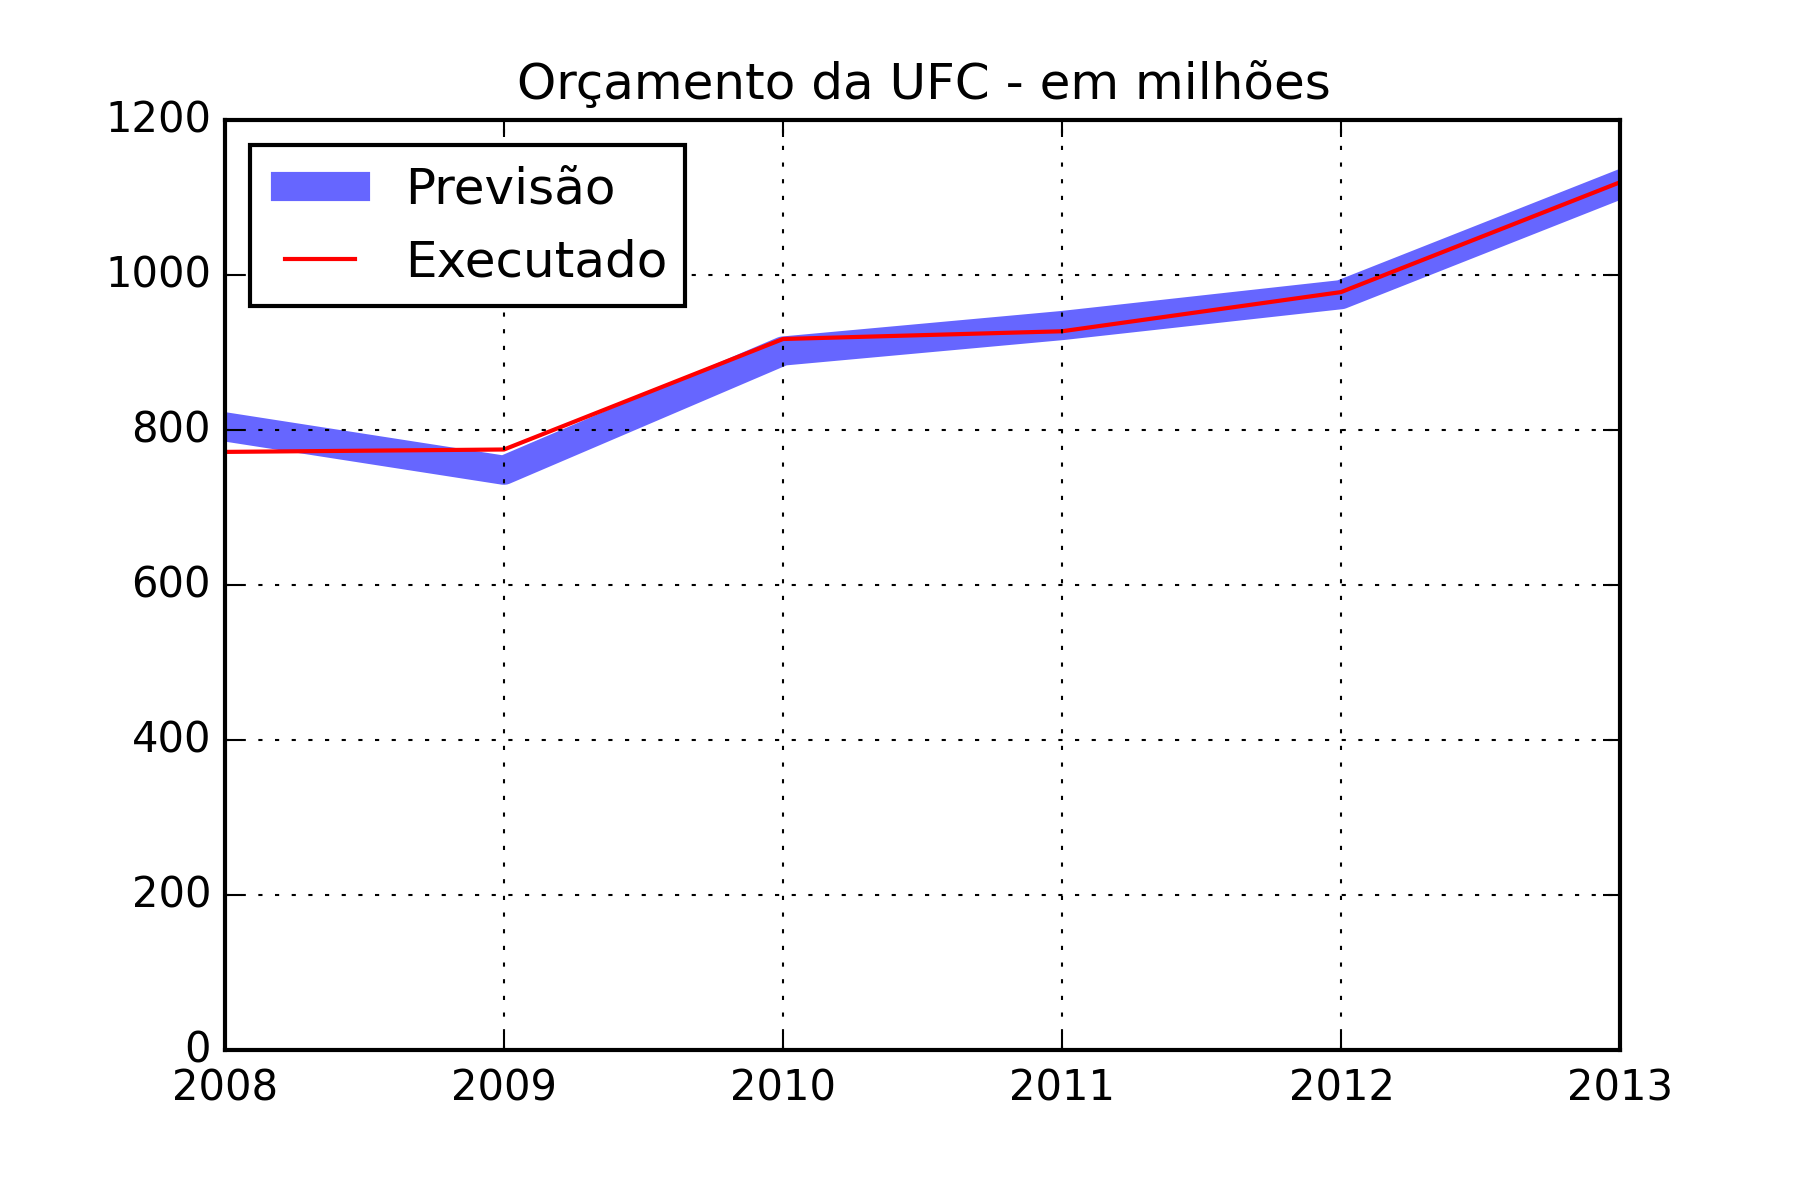
\includegraphics{img/orcamento_ufc.png}
	\caption{Tabela \ref{table:orcamento-ufc}}
	\label{img:orcamento-ufc}
\end{figure}

\subsection{Área construída da UFC}

\begin{figure}[H]
	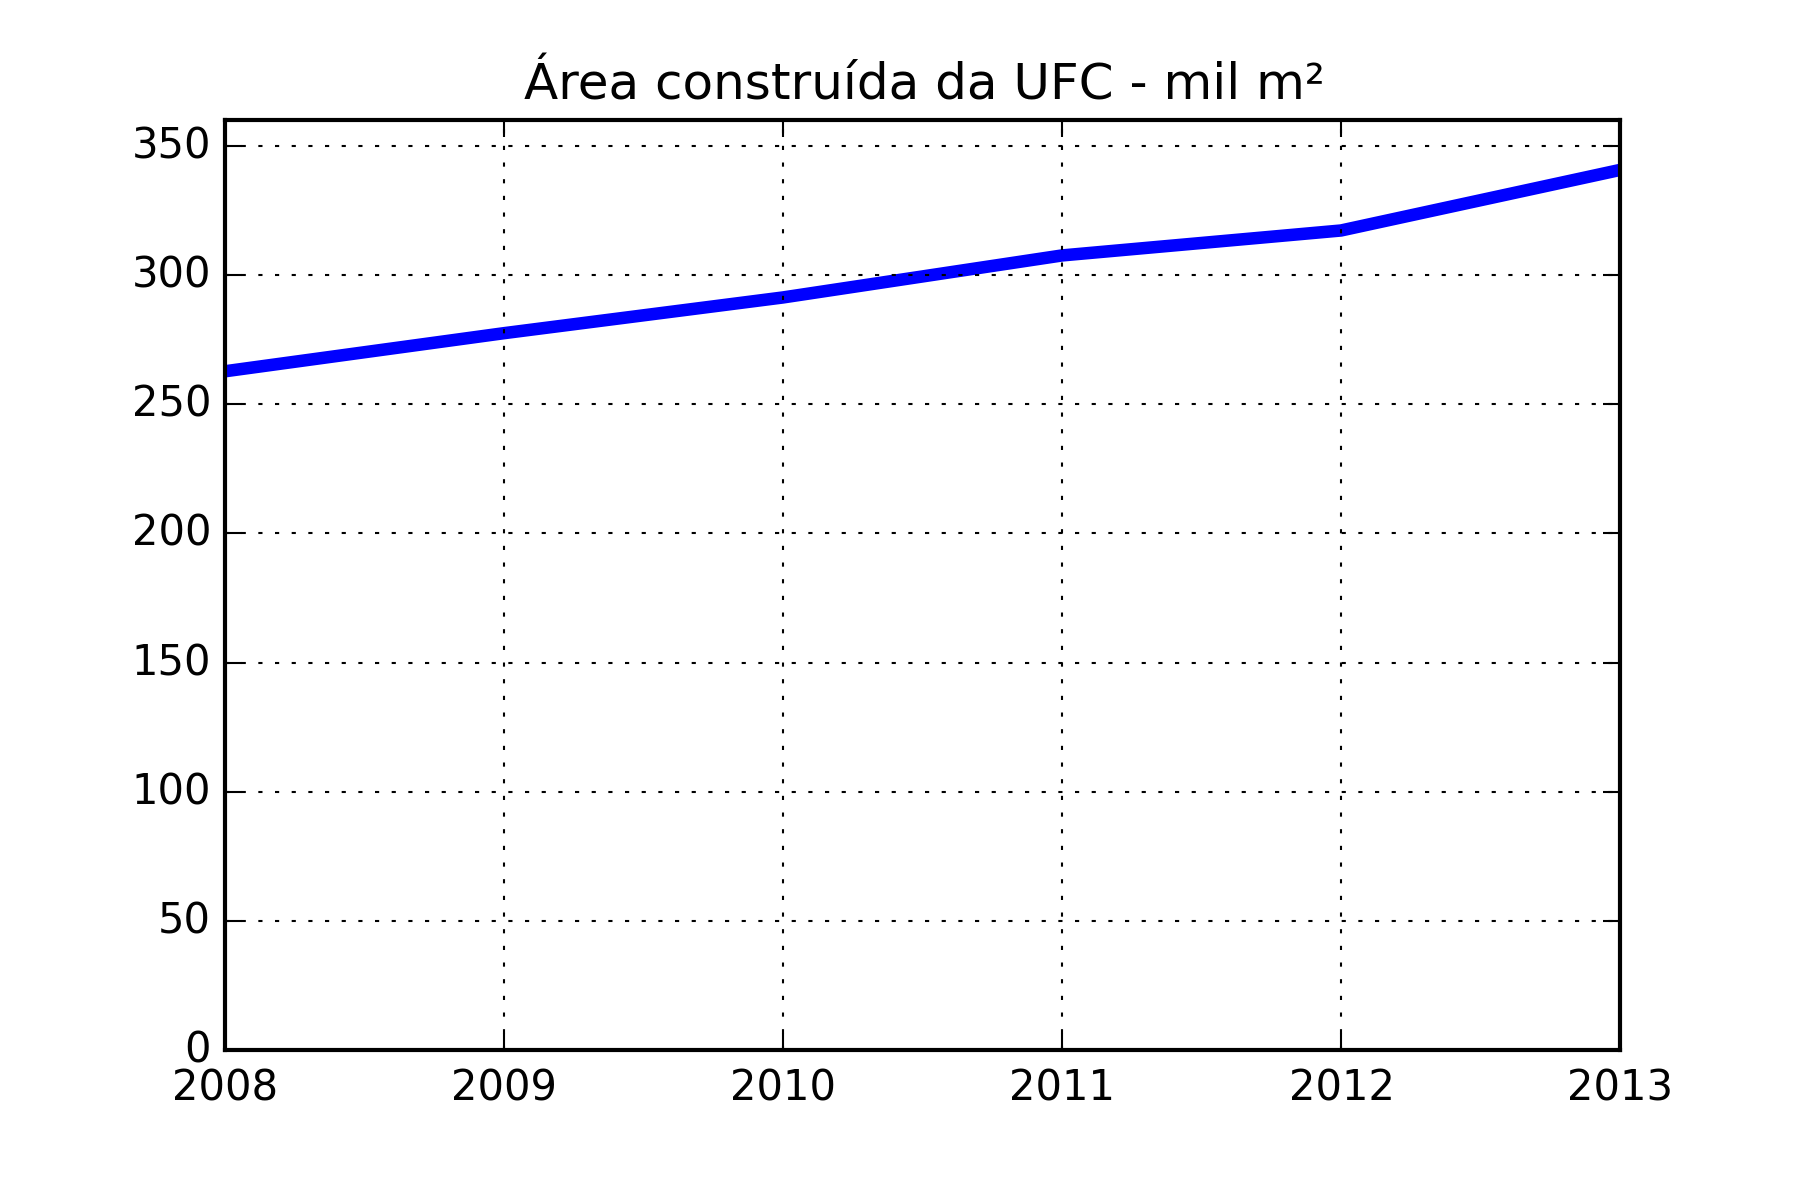
\includegraphics{img/area_construida_ufc.png}
	\caption{Tabela \ref{table:area_construida-ufc}}
	\label{img:area_construida-ufc}
\end{figure}


\subsection{Quantitativos de bolsas para graduação}

\begin{figure}[H]
	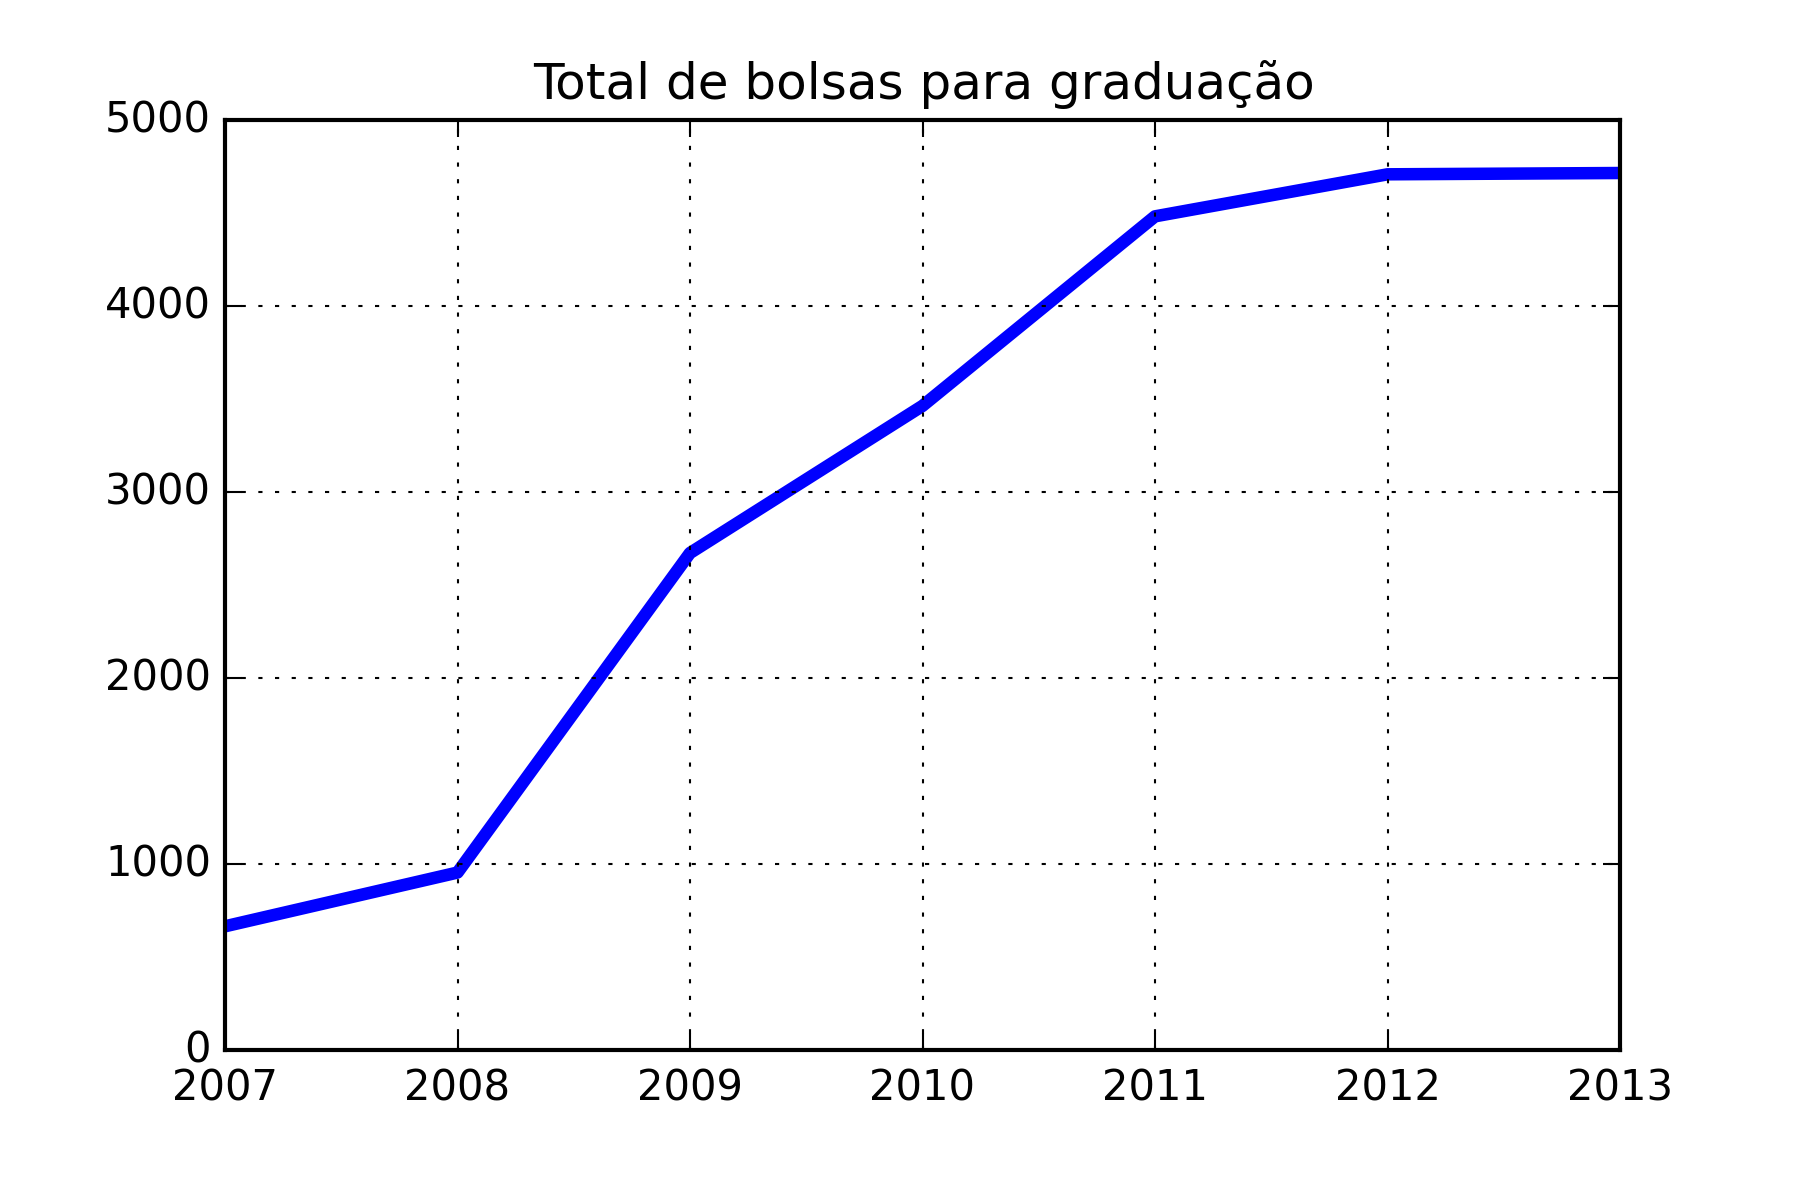
\includegraphics{img/numero_bolsas_graduacao_ufc.png}
	\caption{Tabela \ref{table:numero_bolsas_graduacao-ufc}}
	\label{img:numero_bolsas_graduacao-ufc}
\end{figure}

\subsection{Quantitativos de inscritos(vestibular e sisu) e vagas ofertadas por ano}

\begin{figure}[H]
	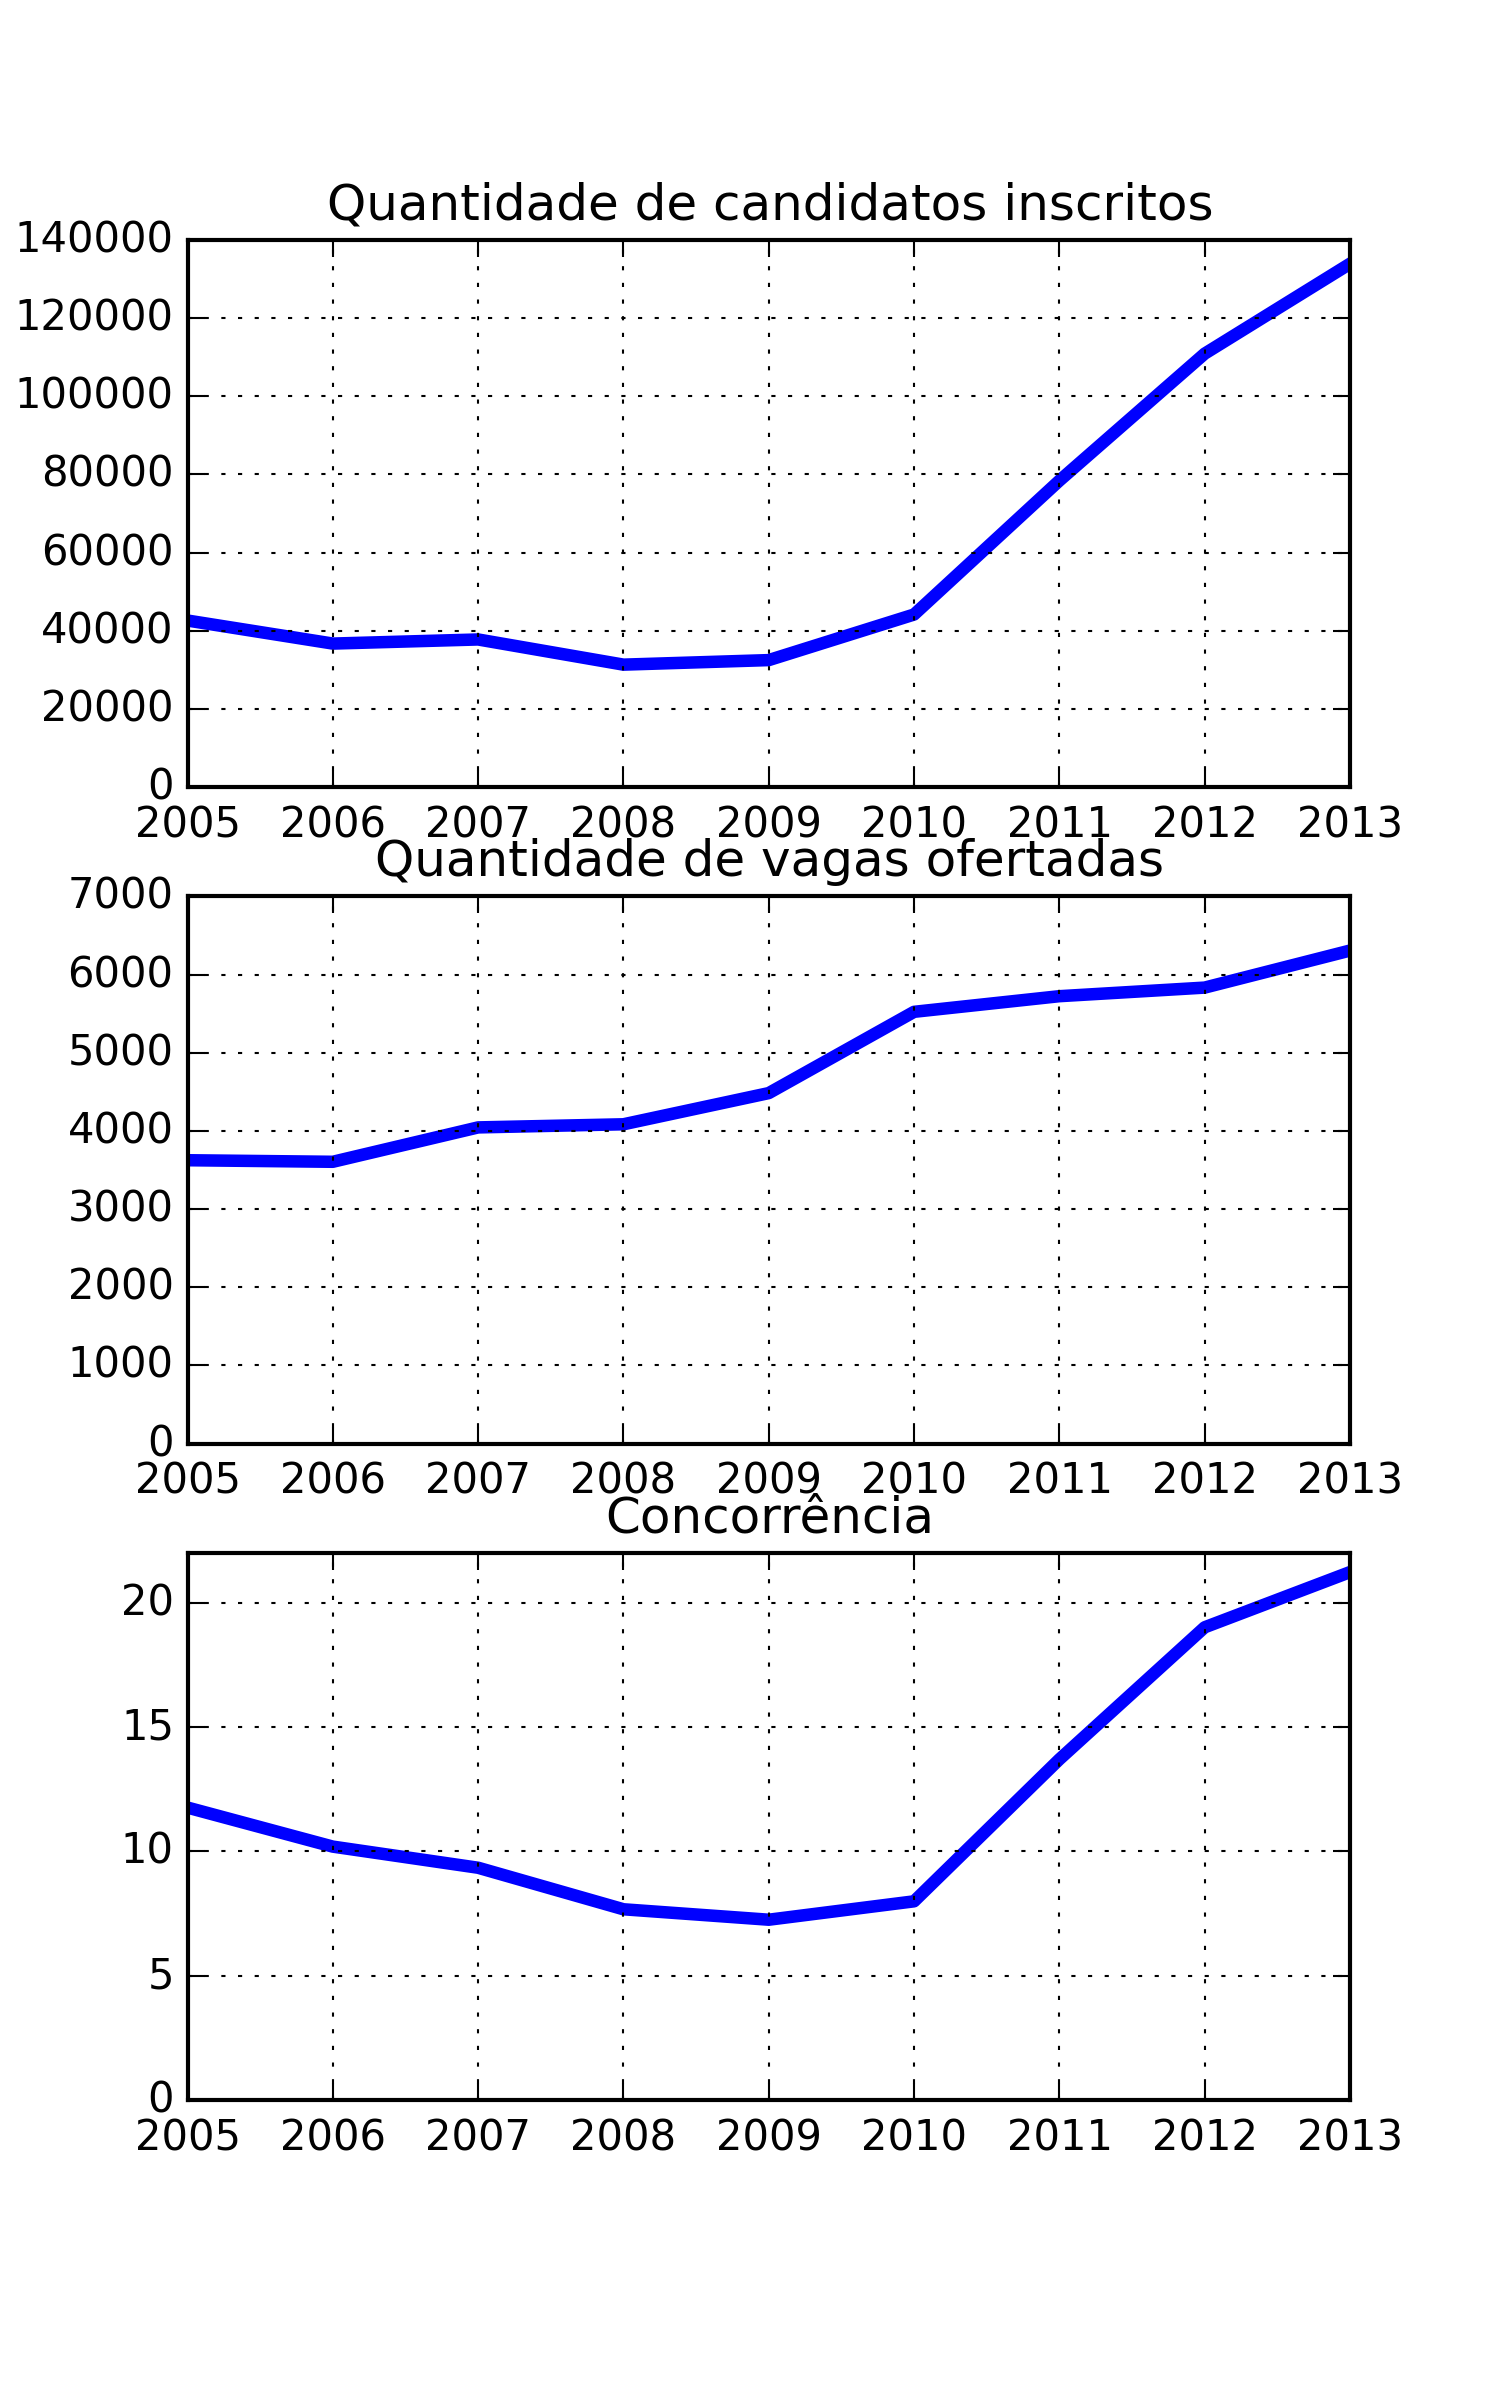
\includegraphics{img/inscritos_ufc.png}
	\caption{Tabela \ref{table:inscritos-ufc}}
	\label{img:inscritos-ufc}
\end{figure}

\subsection{Quantitativo de cursos de graduação por ano}

\begin{figure}[H]
	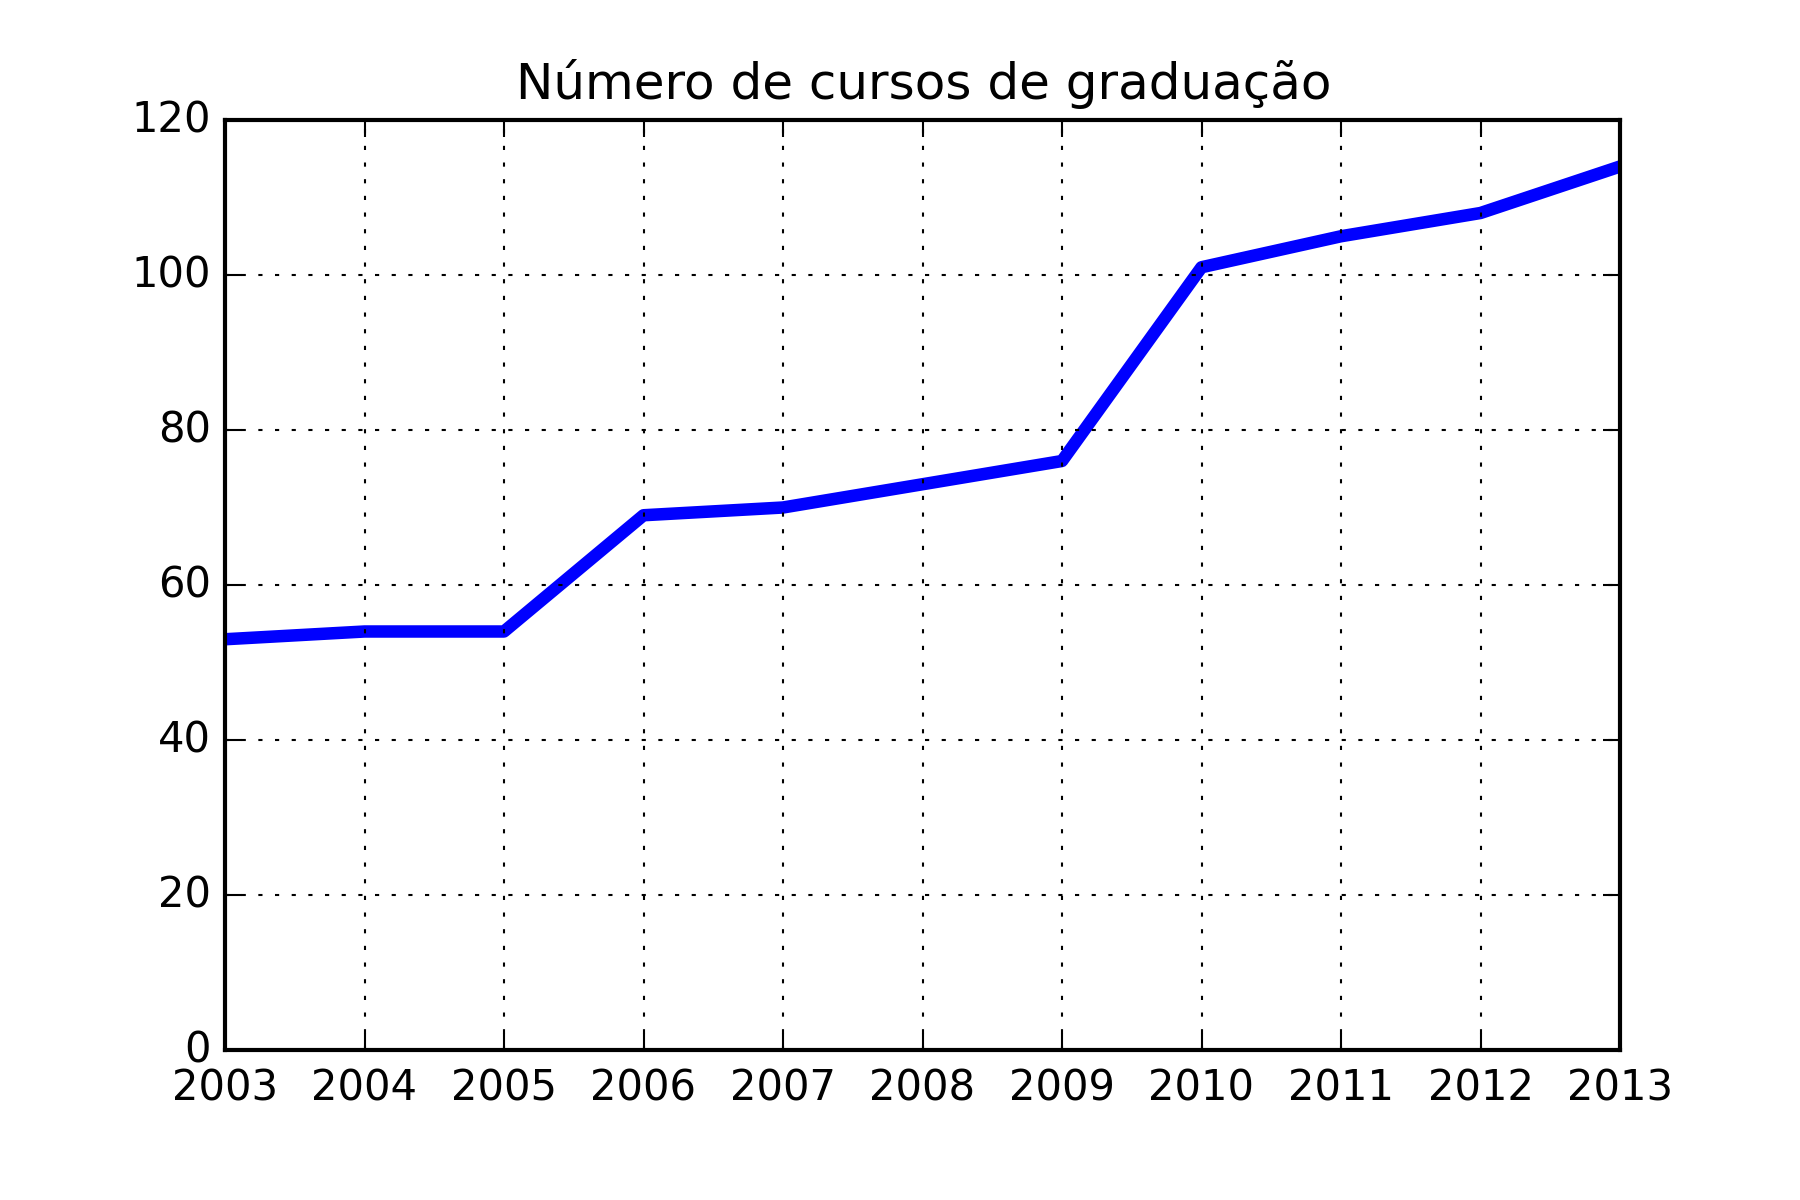
\includegraphics{img/numero_cursos_ufc.png}
	\caption{Tabela \ref{table:numero_cursos-ufc}}
	\label{img:numero_cursos-ufc}
\end{figure}

\subsection{Indicadores de assistência a estudantes}

\begin{figure}[H]
	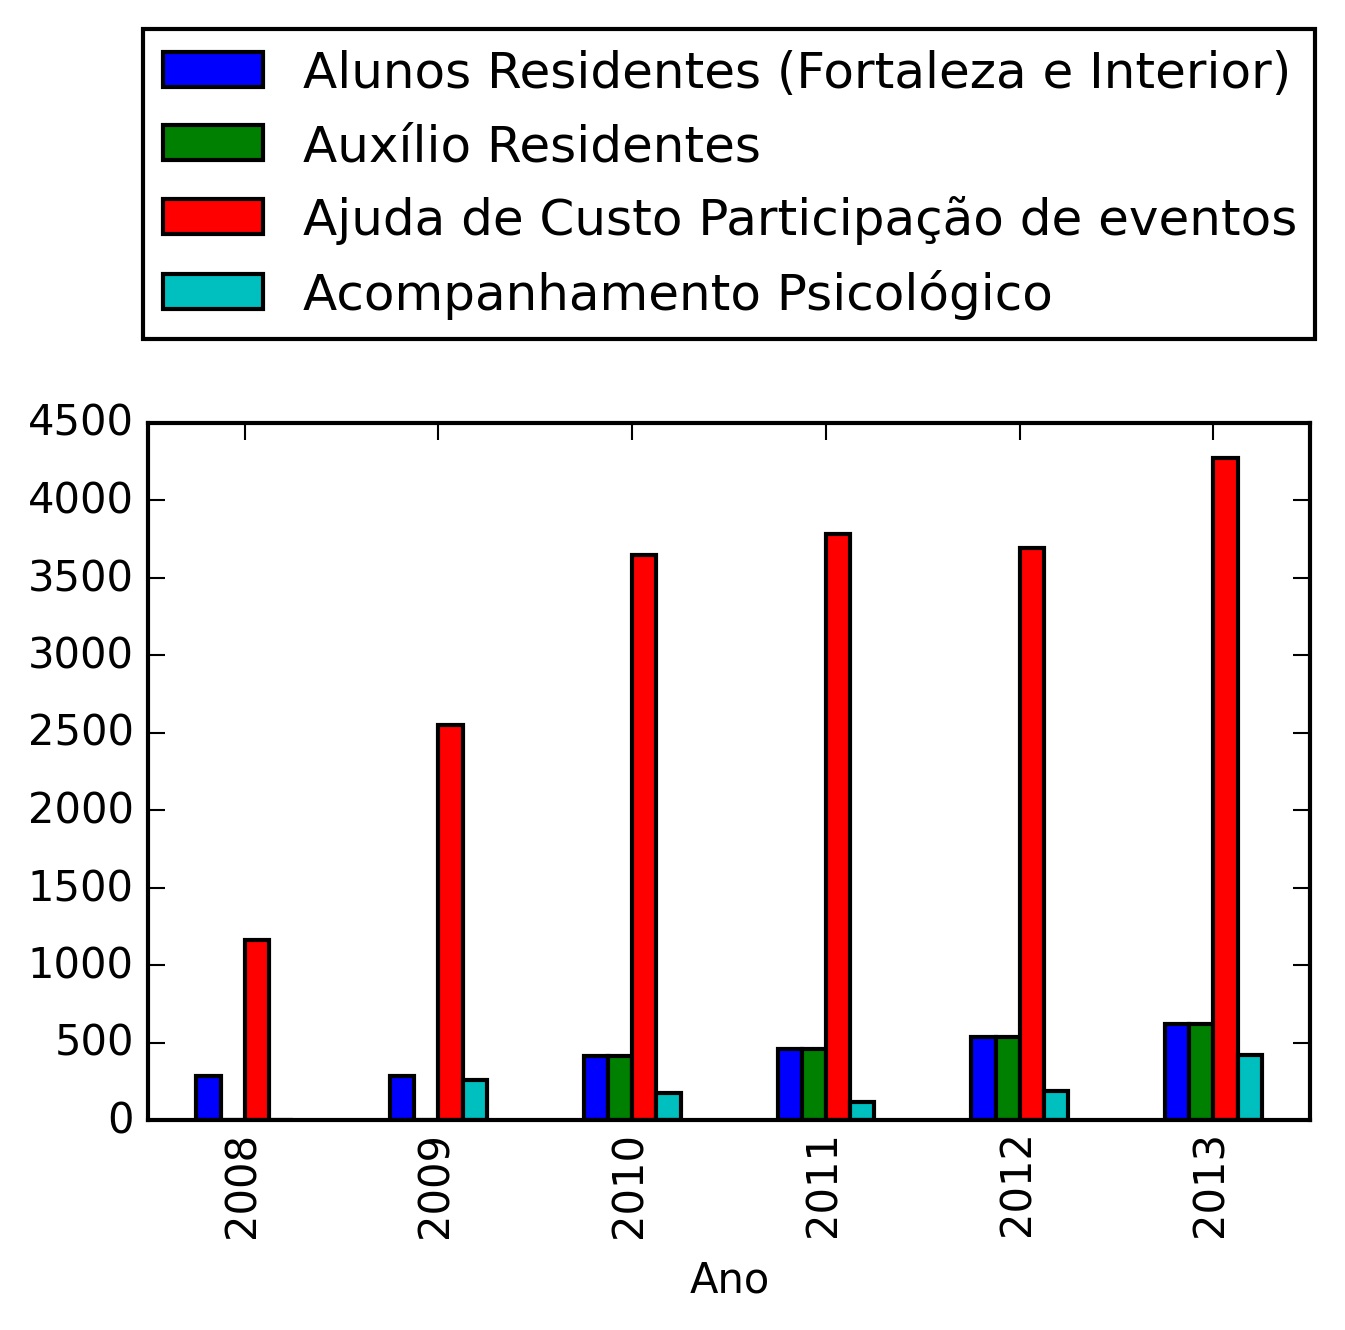
\includegraphics{img/assistencia_ufc.png}
	\caption{Tabela \ref{table:assistencia-ufc}}
	\label{img:assistencia-ufc}
\end{figure}

\subsection{Distribuição de docentes e técnicos-administrativos}

\begin{figure}[H]
	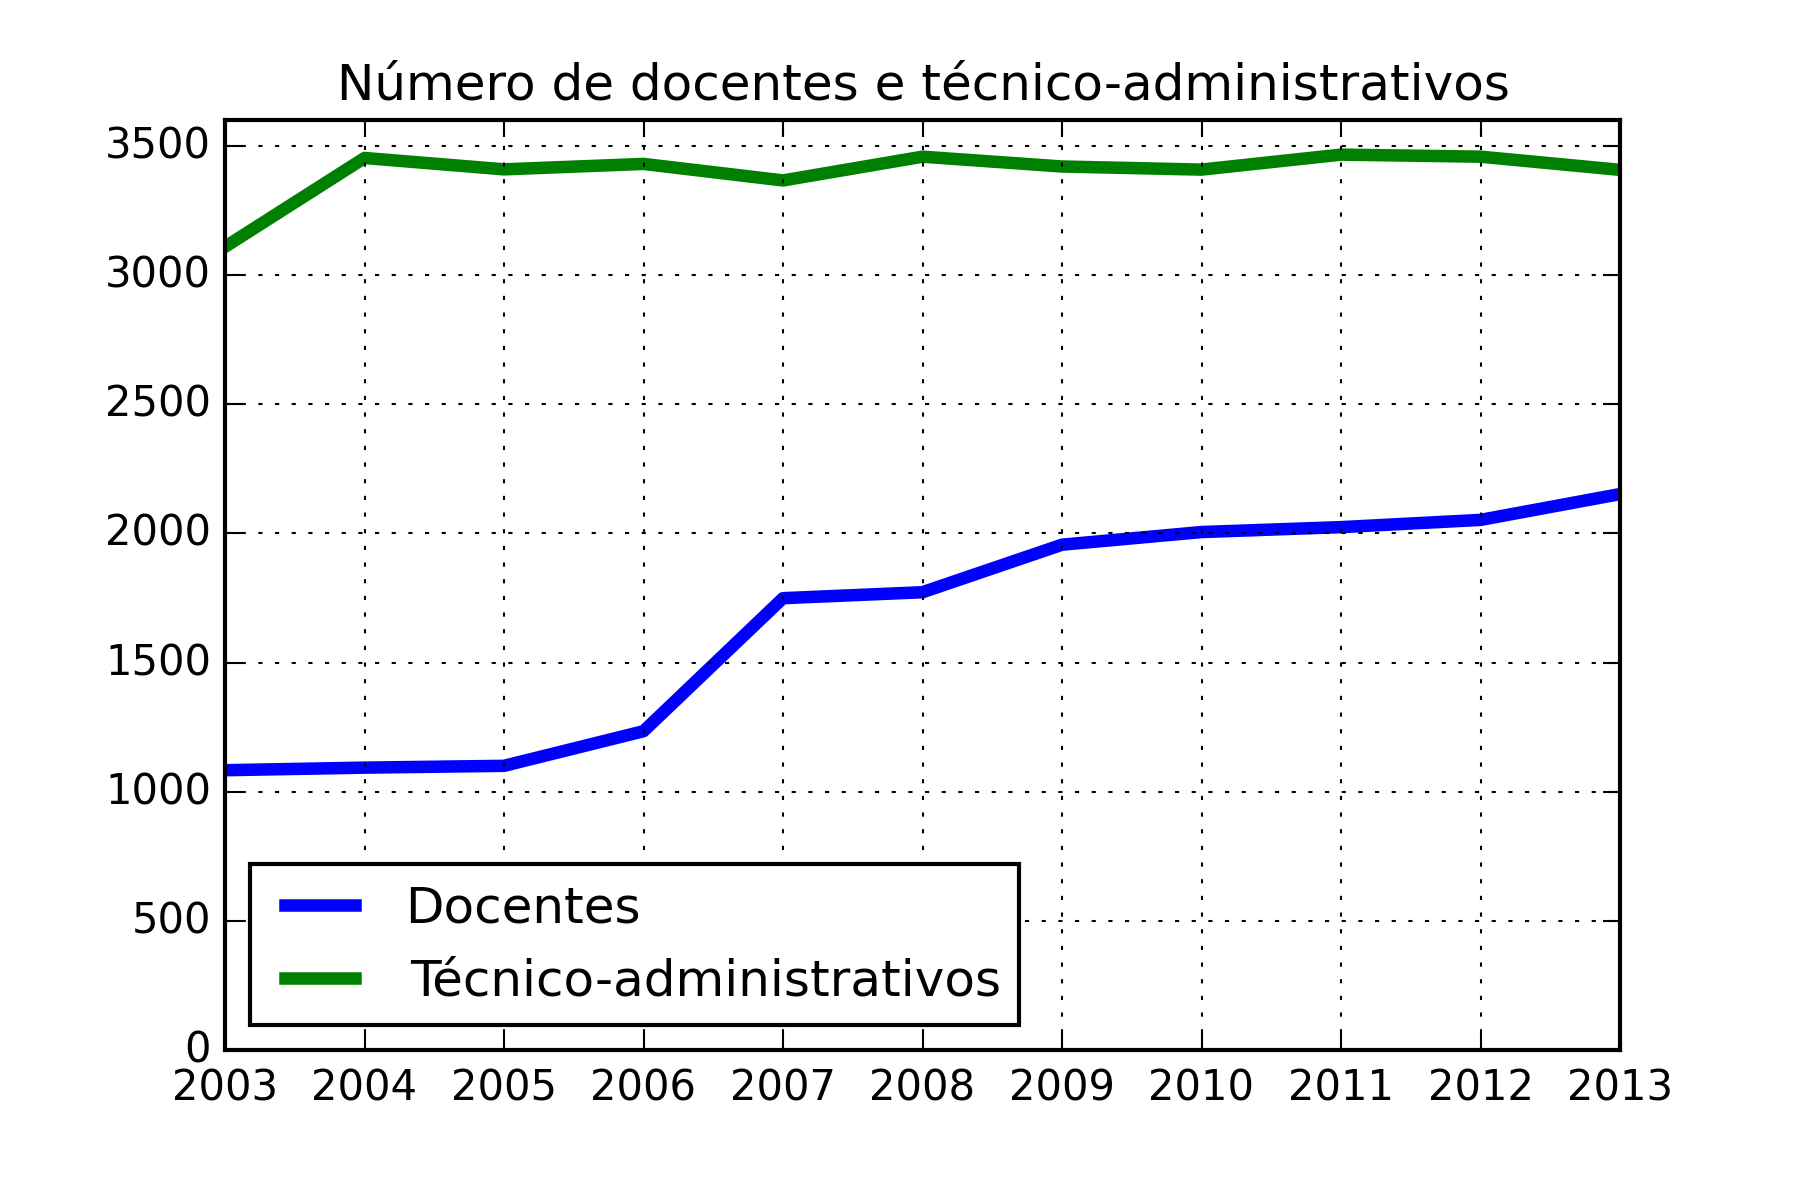
\includegraphics{img/servidores_ufc.png}
	\caption{Tabela \ref{table:servidores-ufc}}
	\label{img:servidores-ufc}
\end{figure}

\subsection{Indicadores de gestão para o TCU}
\cite{indicadores_TCU}

\begin{tabular}{ll}
\toprule
{} &                                                   Indicador \\
\midrule
0  &  AE – Aluno Equivalente da UFC \\
1  &  ATI – Aluno em Tempo Integral \\
2  &  AgE – Aluno Equivalente de Graduação \\
3  &  ApgTI – Aluno da Pós-Graduação em Tempo Integral \\
4  &  ArTI – Aluno de Residência em Tempo Integral \\
5  &  AgTI – Aluno de Graduação em Tempo Integral \\
6  &  Ag – Aluno de Graduação \\
7  &  Apg – Aluno de Pós-Graduação \\
8  &  Ar – Aluno de Residência Médica \\
9  &  Ndi – Alunos Diplomados \\
10 &  Ni – Alunos Ingressantes \\
11 &  Custo corrente com HU (inclui 65\% do HU) \\
12 &  Custo corrente sem HU \\
13 &  Número de funcionários Equivalente com HU \\
14 &  Número de funcionários Equivalente sem HU \\
15 &  Professor Equivalente \\
16 &  I.A. Custo corrente com HU/Aluno Equivalente \\
17 &  I.B. Custo Corrente sem HU/Aluno Equivalente \\
18 &  II. Aluno Tempo Integral/Professor Equivalente \\
19 &  III.A. Aluno Tempo Integral/Funcionário Equivalente com HU \\
20 &  III.B. Aluno Tempo Integral/Funcionário Equivalente sem HU \\
21 &  IV.A. Funcionário Equivalente com HU/Professor Equivalente \\
22 &  IV.B. Funcionário Equivalente sem HU/Professor Equivalente \\
23 &  V. Grau de Participação Estudantil-GPE \\
24 &  VI. Grau de Envolvimento com Pós-Graduação-GEPG \\
25 &  VII. Conceito CAPES para a Pós-Graduação \\
26 &  VIII. Índice de Qualificação do Corpo Docente-IQCD \\
27 &  IX. Taxa de Sucesso na Graduação-TSG \\
\bottomrule
\end{tabular}

\begin{tabular}{lllllll}
\toprule
Ano &          2008 &          2009 &          2010 &          2011 &          2012 &          2013 \\
\midrule
Indic &               &               &               &               &               &               \\
0         &  34023.00 &  33557.62 &  37908.26 &  40708.72 &  41144.35 &  42443.53 \\
1         &  21212.00 &  21461.92 &  23307.93 &  25035.20 &  26330.48 &  26466.34 \\
2         &  28080.00 &  27074.62 &  31631.26 &  33018.72 &  32468.35 &  34247.53 \\
3         &  5615.00 &  6075.00 &  5839.00 &  7308.00 &  8268.00 &  7760.00 \\
4         &  328.00 &  408.00 &  438.00 &  382.00 &  408.00 &  436.00 \\
5         &  15269.00 &  14978.92 &  17030.93 &  17345.20 &  17654.48 &  18270.34 \\
6         &  20991.00 &  21289.00 &  22538.00 &  25971.00 &  26956.00 &  27433.00 \\
7         &  2808.00 &  3038.00 &  2920.00 &  3654.00 &  4134.00 &  3880.00 \\
8         &  164.00 &  204.00 &  219.00 &  191.00 &  204.00 &  218.00 \\
9         &  2520.00 &  2481.00 &  2586.00 &  2792.00 &  2684.00 &  2920.00 \\
10        &  4822.00 &  4731.00 &  6204.00 &  5643.00 &  6406.00 &  6087.00 \\
11        &  444351055.04 &  473411413.49 &  564453156.89 &  581255114.03 &  560737712.22 &  698496687.71 \\
12        &  426930950.49 &  431030343.74 &  513713119.26 &  491835392.86 &  482034252.71 &  609763905.54 \\
13        &  3313.00 &  3252.50 &  3255.50 &  3283.25 &  3281.50 &  3277.75 \\
14        &  1902.25 &  1916.25 &  1954.00 &  1927.00 &  1990.00 &  2047.50 \\
15        &  1619.00 &  1765.50 &  1856.00 &  1851.50 &  1912.50 &  1948.50 \\
16        &  13060.38 &  14107.42 &  14889.98 &  14278.39 &  13628.55 &  16457.08 \\
17        &  12548.36 &  12844.49 &  13551.48 &  12081.82 &  11715.69 &  14366.47 \\
18        &  13.10 &  12.16 &  12.56 &  13.52 &  13.77 &  13.58 \\
19        &  6.40 &  6.60 &  7.16 &  7.63 &  8.03 &  8.07 \\
20        &  11.15 &  11.20 &  11.93 &  12.99 &  13.23 &  12.93 \\
21        &  2.05 &  1.84 &  1.75 &  1.77 &  1.72 &  1.68 \\
22        &  1.17 &  1.09 &  1.05 &  1.04 &  1.04 &  1.05 \\
23        &  0.73 &  0.70 &  0.76 &  0.67 &  0.65 &  0.67 \\
24        &  0.12 &  0.12 &  0.11 &  0.12 &  0.13 &  0.12 \\
25        &  4.13 &  4.11 &  4.22 &  4.22 &  4.20 &  4.34 \\
26        &  3.95 &  3.73 &  4.03 &  4.13 &  4.15 &  4.24 \\
27        &  70.00 &  66.86 &  68.45 &  69.06 &  66.63 &  56.51 \\
\bottomrule
\end{tabular}

\textbf{p. 57~58}

\subsection{Porcentagem de alunos de graduação com bolsas}

\begin{figure}[H]
	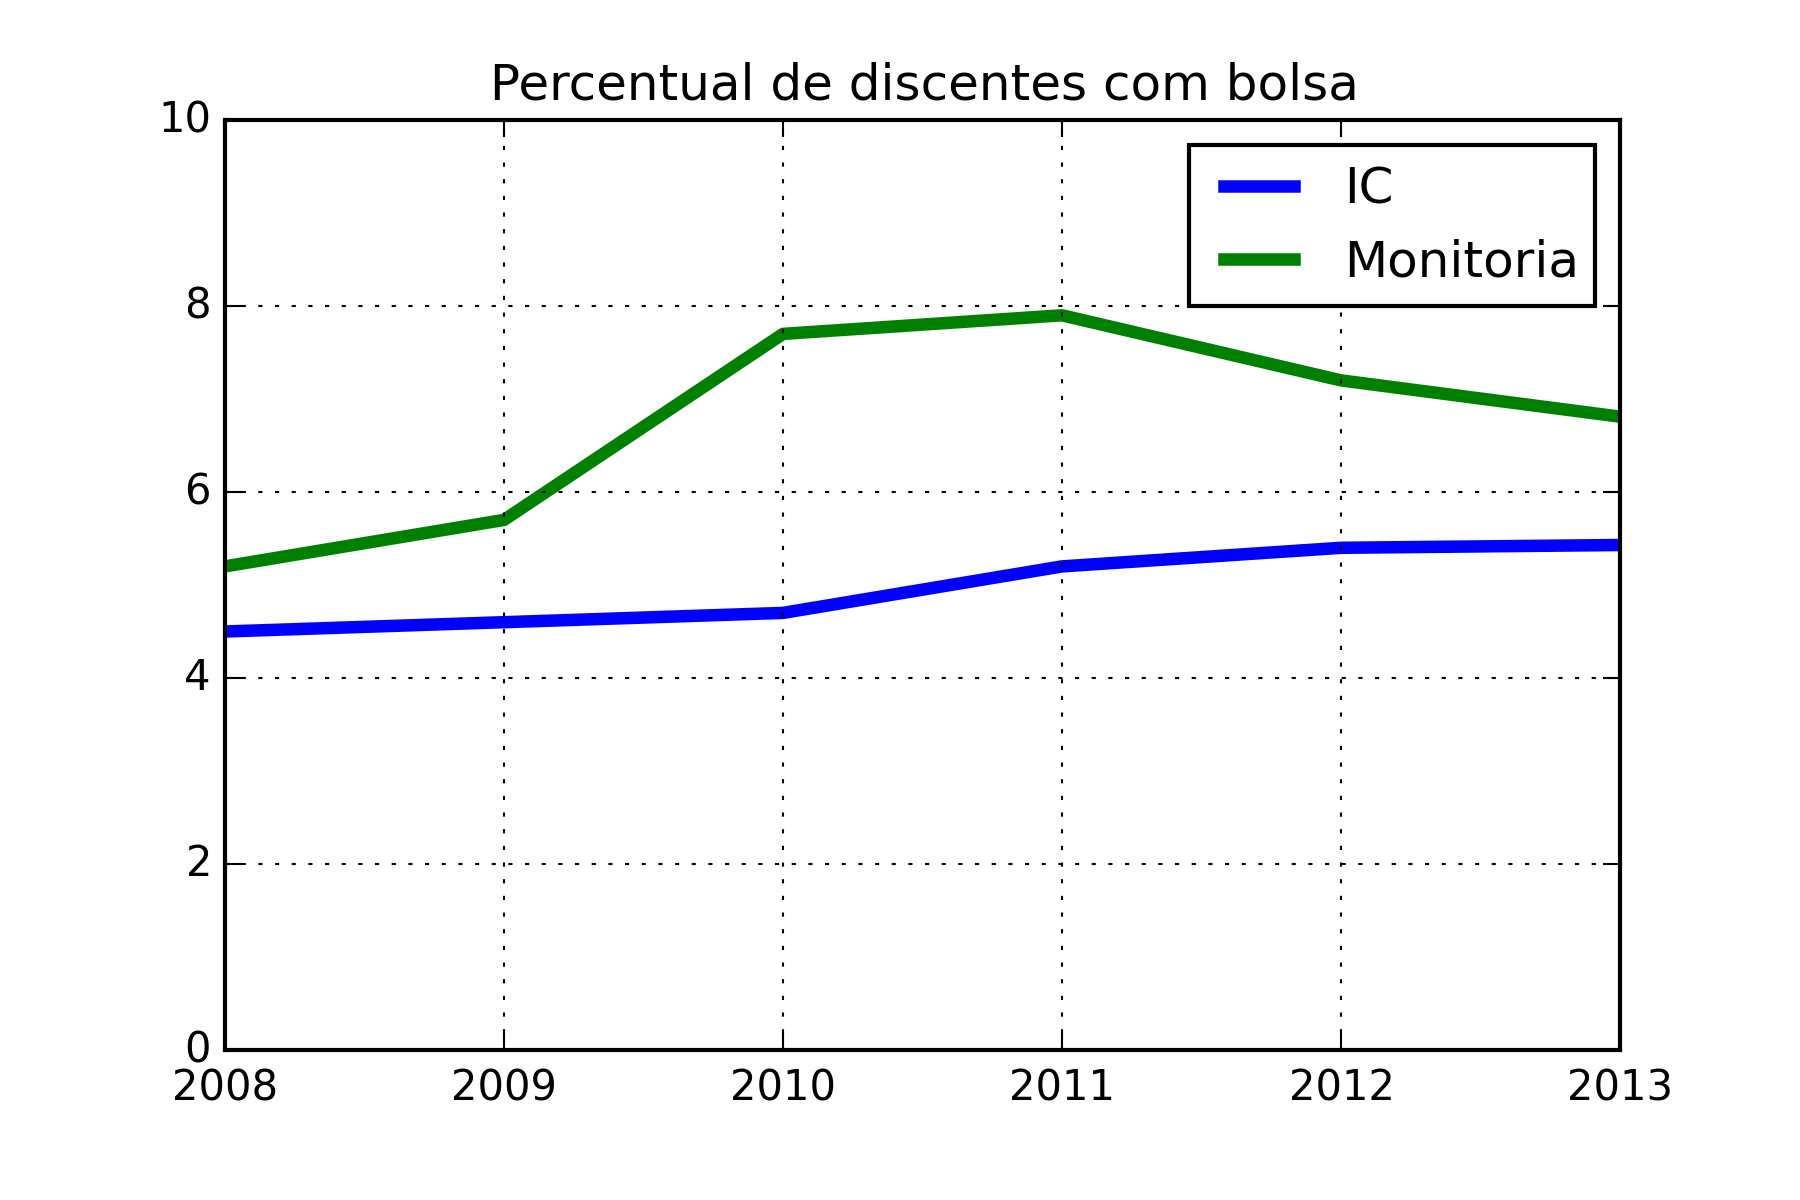
\includegraphics{img/pct_discentes_bolsa_ufc.png}
	\caption{Tabela \ref{table:pct_discentes_bolsas-ufc}}
	\label{img:pct_discentes_bolsas-ufc}
\end{figure}


\chapter{Business objectives}

\begin{itemize}
\item Redução de desperdício financeiro - \cite{evasao_global}
\item Redução de abandonos efetivos subsequentes a abandonos temporários
\item REUNI \cite{reuni}
\item PDI \cite{pdi_ufc}
\item Programa de gestão da atual reitoria \cite{henry}
\end{itemize}

\chapter{Business success criteria}

\cite{anuario_2014_base_2013}
\cite{pdi_ufc}

\chapter{Dados}

\begin{table}[H]
\begin{tabular}{lrrlr}
\toprule
ESPECIFICAÇÃO &  Previsão &  Executado & Evolução do executado &  Executado/Previsão (\%) \\
\midrule
Ano  &           &            &                       &                         \\
2008 &  804.05 &  771.74 &  - &  95.98 \\
2009 &  748.06 &  774.84 &  0.00\% &  103.58 \\
2010 &  901.89 &  917.41 &  0.18\% &  101.72 \\
2011 &  934.76 &  927.40 &  0.01\% &  99.21 \\
2012 &  974.62 &  977.95 &  0.05\% &  100.34 \\
2013 &  1116.86 &  1119.66 &  0.14\% &  100.25 \\
\bottomrule
\end{tabular}
\caption{Anuário estatístico da UFC 2014 base 2013 p. 56}
\label{table:orcamento-ufc}
\end{table}

\begin{table}[H]
\begin{tabular}{lcc}
\toprule
ESPECIFICAÇÃO &  Área Construída (mil m2) & Incremento percentual \\
\midrule
Ano  &                           &                       \\
2003 &  233.63 &  - \\
2004 &  233.63 &  0.00\% \\
2005 &  233.63 &  0.00\% \\
2006 &  235.14 &  0.65\% \\
2007 &  235.14 &  0.00\% \\
2008 &  262.73 &  11.73\% \\
2009 &  277.48 &  5.61\% \\
2010 &  291.31 &  4.98\% \\
2011 &  307.57 &  5.58\% \\
2012 &  317.23 &  3.14\% \\
2013 &  340.67 &  7.39\% \\
\bottomrule
\end{tabular}
\caption{Anuário estatístico da UFC 2014 base 2013 p. 56}
\label{table:area_construida-ufc}
\end{table}

\begin{table}[H]
\begin{tabular}{llrrrrrrr}
\toprule
{} &                               ESPECIFICAÇÃO &  2007 &  2008 &  2009 &  2010 &  2011 &  2012 &  2013 \\
\midrule
0  &                    Aprendizagem Cooperativa &     - &     - &    98 &   226 &   250 &   250 &   233 \\
1  &                        Apoio Administrativo &     - &     - &     - &   100 &   100 &   200 &   170 \\
2  &                              Cultura e Arte &     - &     - &    64 &    64 &    64 &    80 &   100 \\
3  &                                    Desporto &     - &     - &     - &    30 &    50 &   100 &   100 \\
4  &                                    Extensão &     - &     - &   274 &   378 &   618 &   670 &   650 \\
5  &                Iniciação Científica - PIBIC &   665 &   726 &   782 &   769 &   942 &   925 &   914 \\
6  &                  Iniciação Acadêmica - PRAE &     - &     - &   500 &   580 &   826 &   756 &   900 \\
7  &   Iniciação à Docência - Remunerada - PIBID &     - &     - &   442 &   605 &   700 &   788 &   732 \\
8  &                                 Informática &     - &     - &    95 &    95 &   100 &   100 &   100 \\
9  &            Monitoria de Projeto (Graduação) &     - &     - &   137 &   256 &   300 &   299 &   276 \\
10 &   Programa de Educação Tutorial - PET - UFC &     - &    24 &    76 &   156 &   280 &   288 &   288 \\
11 &  Programa de Educação Tutorial - PET - SESu &     - &   204 &   204 &   204 &   252 &   252 &   252 \\
\bottomrule
\end{tabular}
\caption{Anuário estatístico da UFC 2014 base 2013 p. 53}
\label{table:numero_bolsas_graduacao-ufc}
\end{table}

\begin{table}
\begin{tabular}{lrrr}
\toprule
ESPECIFICAÇÃO &  Candidatos Inscritos &  Vagas Ofertadas &  Demanda \\
\midrule
Ano  &                       &                  &          \\
2005 &  42616 &  3625 &  11.76 \\
2006 &  36719 &  3605 &  10.19 \\
2007 &  37771 &  4045 &  9.34 \\
2008 &  31328 &  4085 &  7.67 \\
2009 &  32490 &  4484 &  7.25 \\
2010 &  44156 &  5524 &  7.99 \\
2011 &  78415 &  5724 &  13.70 \\
2012 &  110914 &  5834 &  19.01 \\
2013 &  133923 &  6308 &  21.23 \\
\bottomrule
\end{tabular}
\caption{Anuário estatístico da UFC 2014 base 2013 p. 49}
\label{table:inscritos-ufc}
\end{table}

\begin{table}
\begin{tabular}{lrrrrrrrrrrr}
\toprule
Ano &  2003 &  2004 &  2005 &  2006 &  2007 &  2008 &  2009 &  2010 &  2011 &  2012 &  2013 \\
\midrule
ESPECIFICAÇÃO &       &       &       &       &       &       &       &       &       &       &       \\
Nº de Cursos  &  53 &  54 &  54 &  69 &  70 &  73 &  76 &  101 &  105 &  108 &  114 \\
\bottomrule
\end{tabular}
\caption{Anuário estatístico da UFC 2014 base 2013 p. 50}
\label{table:numero_cursos-ufc}
\end{table}

\begin{table}
\begin{tabular}{lrrrrrr}
\toprule
Ano &  2008 &  2009 &  2010 &  2011 &  2012 &  2013 \\
\midrule
Nº de Residências Universitarias                      & - &  15 &  16 &  16 &  14 &  11 \\
Nº de Alunos Residentes (Fortaleza e Interior)        &  284 &  288 &  416 &  458 &  535 &  622 \\
Nº de Auxílio Residentes (Alunos)                     & - & - &  416 &  458 &  535 &  622 \\
Nº de Ajuda de Custo (Alunos)-Participação de eventos &  1161 &  2552 &  3648 &  3782 &  3695 &  4273 \\
Nº de Bolsas de Iniciação Acadêmica                   & - &  500 &  580 &  826 &  756 &  900 \\
Nº de Bolsas de Incentivo ao Desporto                 & - & - &  30 &  50 &  100 &  100 \\
Nº de Acompanhamento Psicológico                      & - &  259 &  179 &  120 &  190 &  423 \\
\bottomrule
\end{tabular}
\caption{Anuário estatístico da UFC 2014 base 2013 p. 52}
\label{table:assistencia-ufc}
\end{table}

\begin{table}
\begin{tabular}{lrrrrrrrrrrr}
\toprule
{} &  2003 &  2004 &  2005 &  2006 &  2007 &  2008 &  2009 &  2010 &  2011 &  2012 &  2013 \\
\midrule
ESPECIFICAÇÃO          &       &       &       &       &       &       &       &       &       &       &       \\
Docentes               &  1083 &  1093 &  1100 &  1234 &  1749 &  1772 &  1956 &  2005 &  2024 &  2052 &  2152 \\
Técnico-administrativo &  3109 &  3453 &  3409 &  3430 &  3366 &  3458 &  3420 &  3408 &  3466 &  3458 &  3407 \\
\bottomrule
\end{tabular}
\caption{Anuário estatístico da UFC 2014 base 2013 p. 54}
\label{table:servidores-ufc}
\end{table}

\begin{table}
\begin{tabular}{llrrrrrr}
\toprule
{} &                                   ESPECIFICAÇÃO &  2008 &  2009 &  2010 &  2011 &  2012 &  2013 \\
\midrule
0 &  Iniciação Científica - PIBIC e PET(Sesu e UFC) &   4.5 &   4.6 &   4.7 &   5.2 &   5.4 &  5.43 \\
1 &                              Bolsa de Monitoria &   5.2 &   5.7 &   7.7 &   7.9 &   7.2 &  6.81 \\
\bottomrule
\end{tabular}
\caption{Anuário estatístico da UFC 2014 base 2013 p. 53}
\label{table:pct_discentes_bolsas-ufc}
\end{table}

\bibliographystyle{acm}
\bibliography{../../../referencias}

\end{document}
